% !TEX TS-program = pdflatex
% !TEX encoding = UTF-8 Unicode
% arara: pdflatex
\pdfminorversion=7
\documentclass[6pt]{scrreport}

\usepackage[english]{babel}
\usepackage[utf8]{inputenc}

%\documentclass[twoside,8pt]{article}
\usepackage{geometry}
\geometry{paperwidth=105mm,paperheight=74mm,margin=10mm}
\usepackage{graphicx}
%\pagestyle{empty}

\usepackage{titlesec}

\usepackage[hidelinks]{hyperref}
\usepackage{enumitem}
\usepackage[
    type={CC},
    modifier={by-nc-sa},
    version={3.0},
]{doclicense}

\title{Wargame in a Suitcase}
\date{2021\\ November}
\author{Way of Wood}

\setlength{\parindent}{0em}
\setlength{\parskip}{0.5em}

\titleformat{\chapter}[display]
  {\normalfont\sffamily\large\bfseries}
  {\chaptertitlename\ \thechapter}{0em}{\Large}
\titlespacing{\chapter}{0em}{0em}{0.5em}


\titleformat{\section}
  {\normalfont\sffamily\large\bfseries}
  {\thesection}{1em}{}


\begin{document}

\maketitle
\doclicenseThis

These rules are based on Age of Fantasy: Skirmish,  a miniature wargame
by \url{www.onepagerules.com}.

The rules do not come with a specific licsense but the authors give in the following
discussion \url{https://www.reddit.com/r/onepagerules/comments/9xg9u5/question_regarding_license/}
the permission to "go ahead and do whatever you want with them" "as long as you don't claim that the rules are yours or make any profit from them".
I would read that statement as a creative commons attribution non-commercial licsense.


\chapter*{General principles}

The most important rule: Whenever the
rules are unclear use common sense and
personal preference. Have fun!

Quality Tests: Roll one six-sided die,
and if you score the unit‘s quality value
or higher it‘s a success.

Modifiers: Regardless of modifiers, rolls
of 6 are always successes, and rolls of 1
are always fails.

\chapter*{Unit stats}

	\begin{minipage}{0.5\textwidth}
 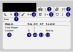
\includegraphics[width=\textwidth]{card-with-numbers.png}
	\end{minipage}
	\begin{minipage}{0.5\textwidth}
    \begin{enumerate}[noitemsep]
      \item Number of models in unit
      \item Cost of the unit
      \item Speed for advancing
      \item Quality / Attack value
      \item Defense value
      \item Wounds / Health
      \item Skills and special rules
      \item Name of the weapon
      \item Range (- is melee)
      \item Number of attacks
      \item Armor piercing
      \item Special rules of weapon
    \end{enumerate}
 	\end{minipage}

\chapter*{Preparation}

  The Battlefield: The game is played on a
  flat 40x40 cm hex grid of 44 by 50 hex fields,
  with at least 15-20 pieces of terrain on it.

  The Armies: The players put together
  two armies of equal cost before the
  game begins (we recommend starting
  with 250pts per player).

  Mission: Place D3+2 objectives. Players
  roll-off to go first, and then alternate in
  placing one marker each outside of
  deployment zones and over 9 hex away
  from each other. At the end of each
  round, if a unit is within 3 hex of a marker
  while enemies aren’t, then it’s seized
  and remains seized even after leaving.
  Stunned units can’t seize markers, and if
  units from both sides are contesting a
  marker then it becomes neutral again.
  The game ends after 4 rounds, and the
  player that controls most markers wins.

  Deployment: Players roll-off, and the
  winner picks one table edge as his
  deployment zone, with his opponent
  taking the opposite. Then the players
  alternate in placing one unit each within
  10 hex of their board edge, starting with the
  player that won the deployment roll-off.

  \chapter*{Playing the Game}

  The game is played in rounds, with
  players alternating in activating one unit
  each, starting with the player that won
  the deployment roll-off. Each new round
  the player that finished activating first
  on the last round gets to start.

  \section*{Activation}

  The player picks one unit and it may do
  one of the following:
  \begin{itemize}
    \item  Hold 0 hex - Can shoot.
    \item  Advance hex according to card - Shoot after moving.
    \item  Rush double move according to card - Can’t shoot.
    \item  Charge double move according to card - Moves into melee.
  \end{itemize}

  \section*{Movement}

  Unit members must be on the adjacent hex field to at least
  another unit. In larger units all but 4 models have to
  be in touch with at least two other models.

  Units may
  may only charge if at least one model
  can reach base contact with one model
  from the target.

  \section*{Shooting}

  Models in range and line of sight may
  fire all weapons, or split their attacks
  evenly among all enemy units within 3”
  of a single model (target picks how).
  Shooting models take one quality test
  per attack, and each success is a hit. For
  each hit defending models roll one die
  trying to score their Defense value or
  higher, and each fail causes one wound.
  Then check the wounds section to see
  what happens to the unit.
  Weapon Profiles: The stats of each
  weapon are shown like this:
  Name (Range, Attacks, Special)
  Weapons with a range value are for
  shooting, and without are for melee.

  \section*{Melee}

  Charging models must move into base
  contact with the target or as close as
  possible, and then defenders must do
  the same by moving up to 3 hex. Models
  within 2 hex of enemies may strike with all
  their melee weapons, which works just
  like shooting (may also split attacks).

  Then the defending unit may choose to
  strike back, however after attacking in
  melee for the first time units only hit on
  unmodified rolls of 6 in any subsequent
  melee, until the end of the round. If one
  of the two units is destroyed the other
  may move by up to 3 hex, else the charging
  units must move back by 1 hex.

  \chapter*{Wounds}

  Whenever a model takes one or more
  wounds place a wound marker next to it
  for each wound. Then roll one die and
  add the number of markers to the result
  to see what happens:
  \begin{itemize}
    \item 2-5: Stunned
    \item 6+: Knocked Out
  \end{itemize}

  Knocked Out: Remove from play.

  Stunned: The model is Stunned until the
  end of its next activation (place it on its
  side to show this). Stunned models fail
  morale tests automatically and must stay
  idle. If a Stunned model takes any hits
  from shooting or is charged again, then
  it is Knocked Out.

  Groups \& Wounds: Whenever a unit
  with multiple models takes wounds,
  each wound kills one model until only
  one last model remains. Only the last
  model accumulates wounds and rolls to
  see if it’s Stunned or Knocked Out.

  \section*{Morale}

  Morale Tests: To take a morale test the
  unit simply takes one Quality test.
  Rout Tests: If at the end of any round an
  army is down to half of its starting units
  or less, then all of its units must take a
  morale test. If the test is failed the unit
  immediately Routs (remove from play).

  \chapter*{Terrain}

  \textbf{Cover Terrain:} Units that shoot at
  enemies with most models in or behind
  cover get -1 to shooting.

  \textbf{Difficult Terrain:} Units moving through
  difficult terrain can’t move more than 6”
  in total at a time.

  \textbf{Dangerous Terrain:} Models moving
  across dangerous terrain or that activate
  in it must roll one die (or as many as
  their tough value), and for each roll of 1
  they take one wound.

\chapter*{Skills}

\textbf{Ambush:} This model may be kept in
reserve instead of deploying. At the start
of any round after the first you may
place the model anywhere over 9” away
from enemy units. If both player have
Ambush they roll-off to see who deploys
first, and then alternate in placing them.

\textbf{Artillery:} Counts as having Defense 2+
against shooting attacks.

\textbf{AP(X):} Targets get -X to Defense rolls
when blocking hits.

\textbf{Blast(X):} All hits are multiplied by X.

\textbf{Deadly(X):} Assign each wound to one
model and multiply it by X. Note that
these wounds don't carry over to other
models if killed.

\textbf{Fast:} Move 9 hex when using Advance and
18 hex when using Rush/Charge.

\textbf{Fear:} Always counts as having dealt +D3
wounds for seeing who won melee.

\textbf{Fearless:} Gets +1 to morale tests.
Fire Breath: Once per round deal either
3 hits with AP(1) in melee, or to one
enemy unit within 12 hex in line of sight.

\textbf{Flying:} May move through obstacles
and may ignore terrain effects.

\textbf{Furious:} Gets +1 attack with a weapon
of your choice when charging.

\textbf{Hero:} May be deployed as part of
friendly units, and they may use his
quality value for morale tests. When
taking hits you must use the defense
value of the hero’s unit until all non-
hero models are killed.

\textbf{Immobile:} May never move/charge.

\textbf{Impact(X):} Deals X automatic hits when
charging successfully.

\textbf{Indirect:} May target enemies that are
not in line of sight and ignores cover
from sight obstructions, but gets -1 to
hit rolls when shooting after moving.

\textbf{Phalanx:} Enemies charging this unit
don’t count as having charged for the
purpose of special rules, and they must
take a dangerous terrain test before
attacking (only roll up to as many dice
as models with phalanx).

\textbf{Poison:} When rolling an unmodified 6
to hit, that hit is multiplied by 3.

\textbf{Regeneration:} When taking a wound,
roll one die. On a 5+ it is ignored.

\textbf{Rending:} Unmodified rolls of 6 to hit
count as having AP(4) and ignore the
regeneration rule.

\textbf{Scout:} This model may be deployed
after all other units, and may then move
by up to 12”, ignoring terrain. If both of
the players have Scout they roll-off to
see who deploys first, and then alternate
in placing and moving them.
Slow: Move 4” when using Advance
and 8” when using Rush/Charge.

\textbf{Sniper:} Shoots at Quality 2+, and may
pick one model in a unit as its target,
which is resolved as if it’s a unit of 1.

\textbf{Stealth:} Enemies get -1 to shooting when
targeting this unit.
Strider: This model may ignore the
effects of difficult terrain.

\textbf{Tough(X):} This model must take X
wounds before being killed. If a model
with tough joins a unit without it, then it
is removed last when the unit takes
wounds. Note that you must continue to
put wounds on the tough model with
most wounds until it is killed, before
starting to put them on the next tough
model (heroes must still be assigned
wounds last).

\textbf{Wizard(X):} May cast one spell during its
activation at any point, before attacking.
Pick a spell and a target in line of sight
and roll D6+X. If the result is equal or
higher than the number in brackets you
may resolve the effects. Enemy wizards
within 18” and line of sight of the caster
may roll D6+X at the same time, and if
their result is higher the spell is blocked.
Wizards may only either try to cast or
try to block a spell each round.

\section*{Command Groups}

Each unit may only have one of each of
the following upgrades.

\textbf{Sergeant:} One model gets +1 to hit when
shooting or in melee (pick one).

\textbf{Musician / Battle Standard:} Always
counts as having dealt +1 wound for
seeing who won melee.

\end{document}
